\chapter{Étude macroscopique de l'aimantation}
\begin{objectif}
	\item Connaître la notion de dipôle magnétique
	\item Connaître les différents types de magnétisme et la notion
	  d'aimantation induite
	\item Connaître les équations qui contrôlent l'évolution spatiale
	  du champ magnétique dans les milieux magnétiques
	\item Savoir décrire un cycle d'hystérésis et donner une explication
          microscopique à ce dernier
\end{objectif}
\section*{Introduction}
Dans ce chapitre, nous allons étudier les propriétés magnétiques des matériaux 
en les abordant d'un point de vue macroscopique. Quelques rares matériaux 
sont capables de générér leur propre champ magnétique (les aimants par exemple).
On dit alors qu'ils possèdent une \textbf{aimantation permanente}.
La plupart du temps leurs propriétés magnétiques
ne se manifestent que sous l'action d'un champ magnétique produit par une autre source
(une boussole par exemple). Ils se mettent alors à produire un champ propre qui
perturbe le champ dans lequel ils baignent initialement. 
On dit que ces matériaux possèdent une \textbf{aimantation
induite}.
\section{Le dipôle magnétique}
	Lorsqu'un observateur se trouve loin d'un circuit filiforme, il devient insensible
	aux caractéristiques géométriques de ce dernier. Le champ magnétique perçu par ce 
	dernier ne dépendra plus de la taille de la spire ou de sa forme. La spire 
	pourra alors être considéré comme un \textbf{dipôle magnétique}.

	\begin{defn}[Dipôle magnétique]
		Un dipôle magnétique est une source de champ magnétique (aimant 
		ou circuit parcouru par un courant $I$) de dimension typique $a$
		vu de loin, c'est-à-dire depuis une distance $r \gg a$.
	\end{defn}

	\begin{rema}
		De la même manière, deux particules portant une charge opposée
		peuvent être assimilées à grande distance à un dipôle électrique.
	\end{rema}
	
	Nous allons voir que ce modèle est très utile lorsqu'il s'agit de décrire
	le comportement magnétique de la matière. 
	
	\subsection{Champ magnétique d'une spire}
	Pour illustrer le notion de dipôle magnétique,
	nous considérons maintenant une spire de rayon $a$ parcourue par un courant $I$
	(voir Fig.~\ref{fig:aimant_spire}).
	L'idée est de calculer une approximation du champ généré par cette spire
	à une distance $r \gg a$. On considère un point $M$ situé dans le plan 
	$(O, \ey, \ez)$ et reperé par ses coordonnées polaire $(r, \theta)$, 
	où $\theta$ est l'angle entre $\ey$ et $\er$.

	\begin{figure}[htpb]
		\centering
		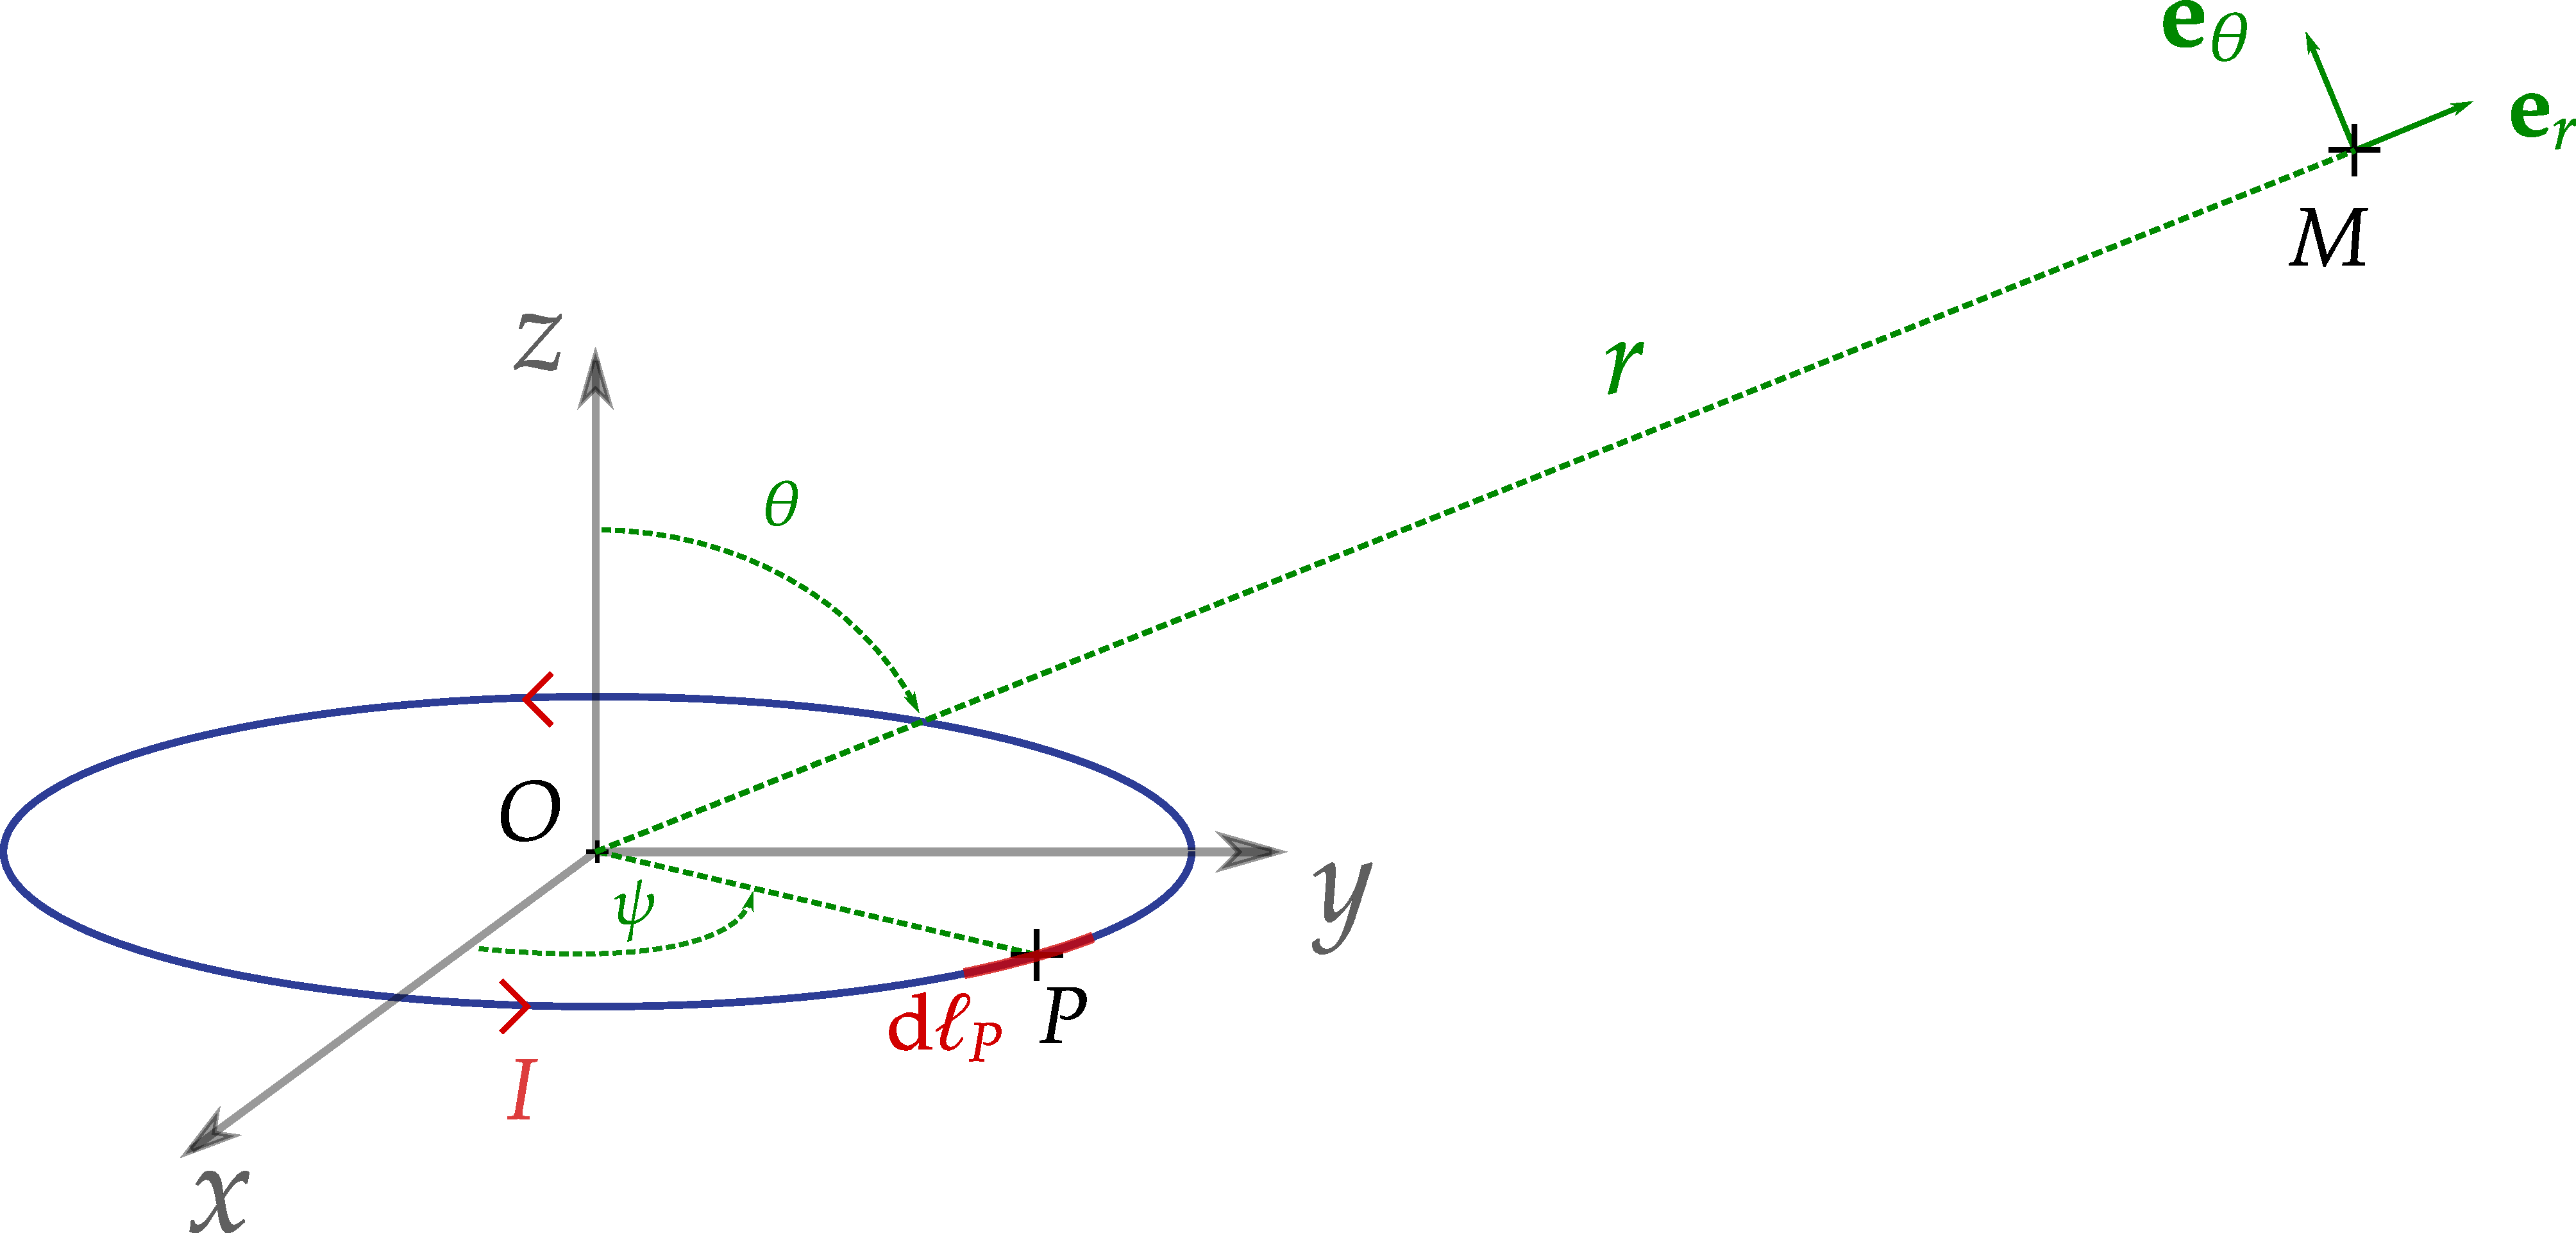
\includegraphics[]{aimant_spire}
		\caption{}%
		\label{fig:aimant_spire}
	\end{figure}

	Le champ magnétique $\mathrm{\textbf{d}}\vecb_P(M)$ généré par l'élément $\dl_P$ 
	de la spire en $M$ est obtenu grâce à loi de Biot et Savart
	\begin{equation*}
		\mathrm{\textbf{d}}\vecb_P(M) = \dfrac{\mu_0}{4 \pi} 
			\dfrac{I \dl_P \wedge \mitbf{PM}}{PM^3}.
	\end{equation*}
	Dans la base $(0, \ex, \ey, \ez)$, $\dl_P = a \mathrm{d}\psi \left(
	- \sin \psi \ex + \cos \psi \ey \right)$ et
	\begin{equation*}
		\mitbf{PM} = \mitbf{PO} + \mitbf{OM}  
		= -a \cos \psi \ex + \left(r\sin \theta - a \sin \psi\right)\ey +
		     r \cos \theta \ez.
	\end{equation*}
	
	Il ne nous reste plus qu'à exprimer $PM^3$. Nous allons nous servir du
	fait que $r \gg a$ pour obtenir un expression approchée de $PM^3$ en 
	réalisant un développement limité. On a alors
	\begin{equation*}
		PM^3 = \left[a^2\cos^2\psi + \left(r \sin \theta - a\sin \psi\right)^2 
		+ r^2 \cos^2 \theta \right]^{3/2}
		= r^3 \left[ 1 - 2\sin \theta \sin \psi \dfrac{a}{r} + \dfrac{a^2}{r^2}
		\right]^{3/2}.
	\end{equation*}
	Comme $r \gg a$, on peut alors réaliser un développement limité à l'ordre $1$
	pour obtenir l'expression de $PM^{-3}$
	\begin{equation*}
		PM^{-3} = r^{-3}\left[1 + \dfrac{3a\sin\theta\sin\psi}{r} +
		          o\left(\dfrac{a}{r}\right)\right] \approx
			  r^{-3} \left(1 + \dfrac{3a\sin\theta\sin\psi}{r}\right)
	\end{equation*}
	Cette expression nous montre que $PM^3$ est égale à $OM^3$ à des termes en
	$a/r$ près. L'approximation dipolaire conduit à considérer que le point $P$
	et le point $O$ sont quasiment confondus pour l'observateur en $M$.
	Finalement, le champ magnétique $\vecb(M)$ généré par la spire en $M$
	s'écrit
	\begin{equation*}
		\vecb(M) \approx \dfrac{\mu_0 Ia}{4 \pi r^3}
		\int_0^{2\pi}\left(1 + \dfrac{3a\sin\theta\sin\psi}{r}\right)
		\left[r \cos\psi\sin\theta\ex -r\sin\psi\cos\theta\ey
		+ \left(a -r)\sin\theta\sin\psi\right)\ez\right]\mathrm{d}\psi.
	\end{equation*}
	On commence par calculer l'intégrale qui va nous permettre d'obtenir la composante
	selon $\ex$ du champ magnétique. Cela donne
	\begin{equation*}
		\int_0^{2\pi} \left(1 + \dfrac{3a \sin\theta\sin\psi}{r}\right)
		\cos\psi \mathrm{d}\psi = \left[\sin \psi + 
		\dfrac{3a\sin\theta\sin^2\psi}{2r} \right]^{2\pi}_0 = 0.
	\end{equation*}
	La composante selon $\ey$ est obtenue en calculant l'intégrale
	\begin{equation*}
		\int_0^{2\pi} \left(1 + \dfrac{3a \sin\theta\sin\psi}{r}\right)
		\sin \psi \mathrm{d}\psi = \left[-\cos \psi + 
			\dfrac{3a\sin\theta}{r}\left(\dfrac{\psi}{2}
			- \dfrac{\sin(2\psi)}{4}\right) \right]^{2\pi}_0 =
			\dfrac{3 \pi a \sin \theta}{r}.
	\end{equation*}
	Finalement, on obtient la composante selon $\ez$ en calculant
	\begin{equation*}
		\begin{array}{rcl}
		\displaystyle \int^{2\pi}_0 \left(1 + \dfrac{3a \sin\theta\sin\psi}
		{r}\right)
		\left(a - r\sin\theta\sin\psi \right)\mathrm{d}{\psi}
		&=& \left[ a \psi + r\sin\theta\cos\psi - 
		\dfrac{3a^2\sin\theta\cos\psi}{r}\right]^{2\pi}_{0} \\ 
		&-& \left[3a\sin^2\theta
		\left(\dfrac{\psi}{2} - \dfrac{\sin(2\psi)}{4}\right)
	\right]^{2\pi}_0 \\[1.5em]
		&=& 2\pi a - 3\pi a \sin^2\theta.
		\end{array}
	\end{equation*}
	Après ce calcul fastidieux on aboutit enfin à l'expression du champ magnétique
	$\vecb(M)$
		\begin{equation*}
			\vecb(M) = \dfrac{\mu_0 I \pi a^2}{4 \pi r^3}
			\left[3\cos\theta\sin\theta\ey + \left(2 - 3 \sin^2\theta\right)\ez
			\right].
		\end{equation*}
	Dans les deux composantes non nulles du champ magnétique, on voit apparaître
	la surface de spire $\pi a ^2$. On définit alors le moment dipolaire $\vecm$
	de la spire $\vecm = \pi a^2 I \ez$ où $\pi a^2 \ez$ est le vecteur surface de la 
	spire orienté par le sens du courant. Finalement, on aboutit à l'expression du champ
	magnétique dans le repère polaire

		\begin{equation}
			\boxed{\vecb(M) = \dfrac{\mu_0 m}{4 \pi r^3} 
			\left[2\cos\theta\er - \sin \theta\etheta\right]}
		\end{equation}

	\begin{defn}[Moment magnétique]
		Soit un circuit filiforme parcourue par un courant $I$ et ayant 
		un vecteur surface $\vecs$ orienté grâce au sens du courant. On 
		définit le moment magnétique $\vecm$ du circuit par
		\begin{equation*}
			\vecm = I\vecs.
		\end{equation*}
		Le moment magnétique s'exprime donc en $\ampere \usk
		\meter \squared$.

		Dans l'approximation dipolaire, le champ magnétique $\vecb$ créé au point
		$M$ de coordonnées $(r, \theta)$, dans le repère polaire centré 
		sur le circuit, est approximativement
		\begin{equation*}
			\vecb(M) = \dfrac{\mu_0 m}{4 \pi r^3} 
			\left[2\cos\theta\er - \sin\theta\etheta\right]
			= \dfrac{\mu_0}{4 \pi} \dfrac{3(\vecm \cdot \er)\er - \vecm}
			{r^3}
		\end{equation*}
	\end{defn}
	
	\subsection{Topologie d'un champ magnétique dipolaire}
	On cherche maintenant à décrire la topologie d'un champ magnétique
	dipolaire. Pour ce faire, on détermine l'équation de ses lignes de champs.

	On considère un moment magnétique $\vecm$ colinéaire à $\ez$. On se place
	dans un repère sphérique $(O, \er, \etheta, \ephi)$ centré sur $\vecm$ 
	(voir Fig.~\ref{fig:aimant_moment_spire}). 
	\begin{figure}[htpb]
		\centering
		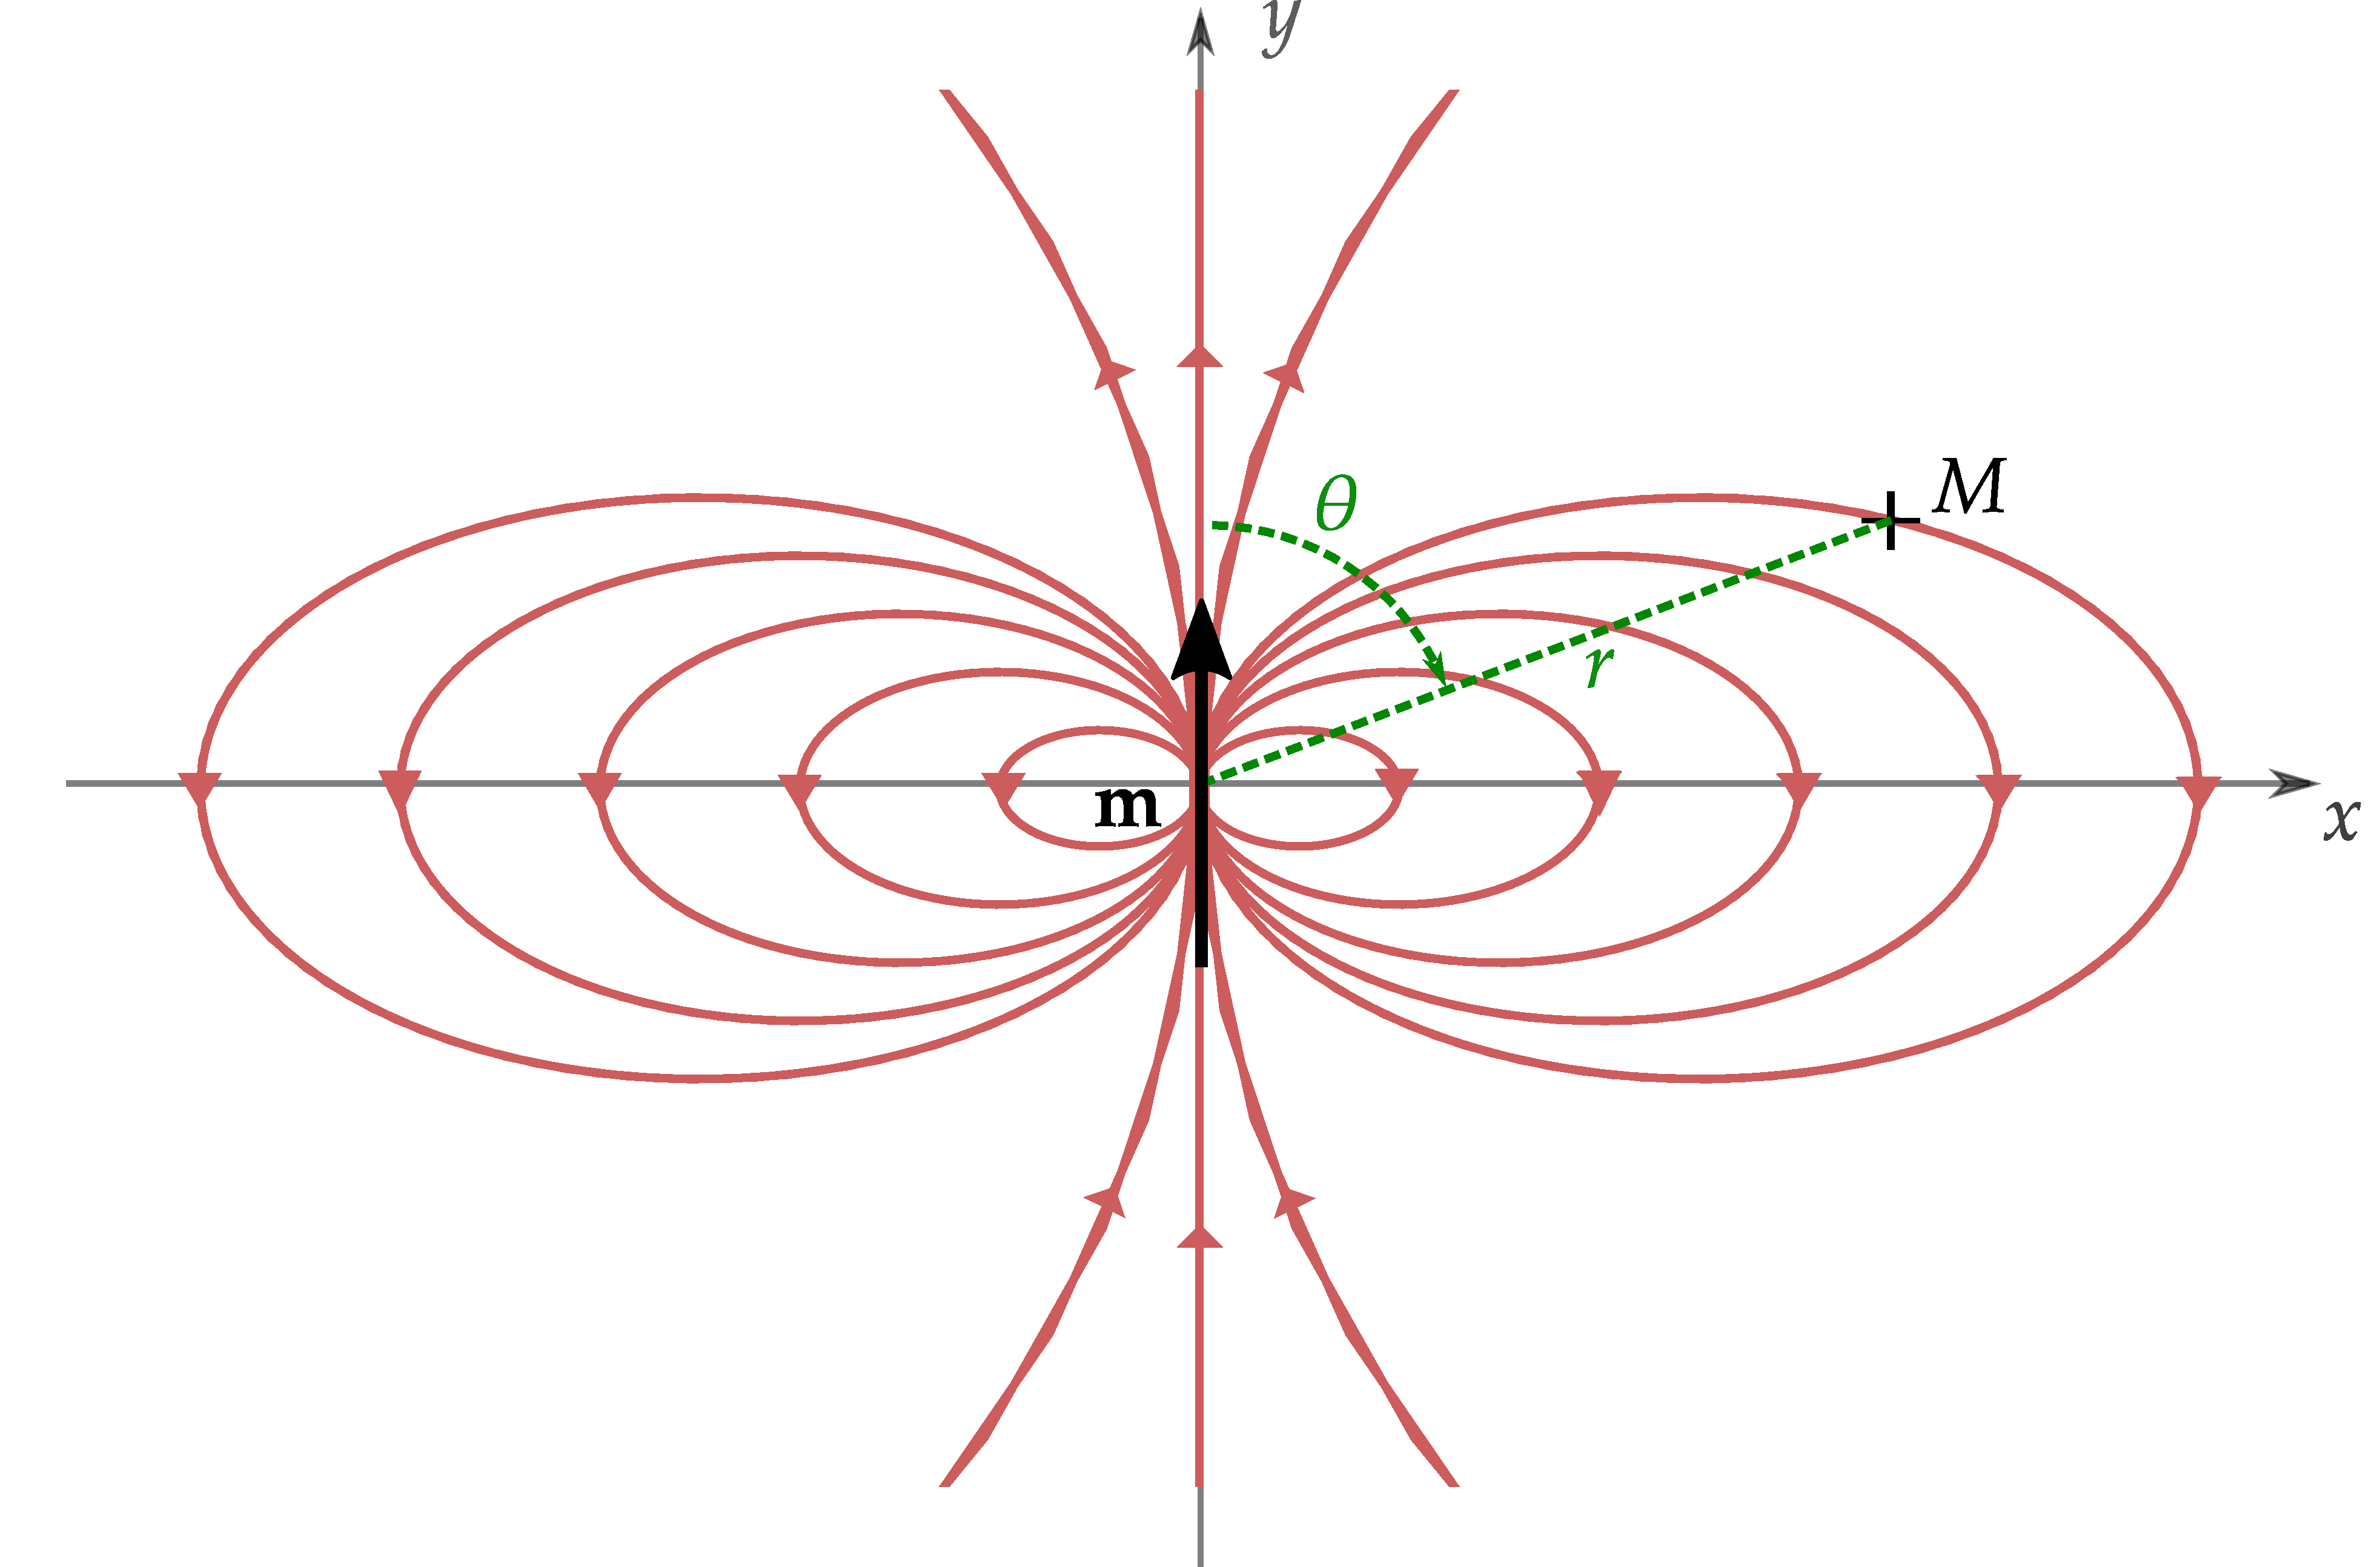
\includegraphics[scale=1]{moment_spire}
		\caption{Champ magnétique généré par un moment dipolaire 
		magnétique. Les lignes rouges représentent les lignes de ce 
		champ.}%
		\label{fig:aimant_moment_spire}
	\end{figure}
	
	Le système présentant
	une symétrie de révolution, nous nous plaçons ici dans un plan méridional,
	ce qui nous permet d'ignorer la coordonnée $\phi$. Un point
	$M$ de l'espace est donc répéré par ses coordonnées $(r, \theta)$. L'équation des
	lignes de champ est obtenue en écrivant qu'en tout point $M$, l'élément 
	de ligne $\dl$ centré en $M$ vérifie
	\begin{equation*}
		\vecb(M) \wedge \dl = \mitbf{0} \iff \dfrac{\dr}{B_r} = 
		\dfrac{r\dtheta}{B_\theta} \iff \dfrac{\dr}{2\cos\theta} =
		\dfrac{r \dtheta}{\sin \theta} \iff \boxed{r = r_0 \sin^2 \theta,}
	\end{equation*}
	où $B_r$ et $B_\theta$ sont respectivement les composantes de $\vecb$ selon
	$\er$ et $\etheta$ et $r_0$ le rayon de la ligne de champ en $\theta = 
	\dfrac{\pi}{2}$. Ces lignes sont représentées en rouge sur la 
	figure~\ref{fig:aimant_moment_spire}. Sur cette figure, l'orientation
	de $\vecm$ définit les pôles Nord et Sud de la spire.
	
	\begin{rema}
	L'étude des lignes
	de champ dans un repère 2D suffit ici car le système présente une symétrie de
	révolution autour de l'axe $z$. 
	\end{rema}

	\begin{defn}[Pôles magnétiques]
		Les lignes de champ magnétique quittent le pôle Nord et 
		reviennent par le pôle Sud.
	\end{defn}
	
	\begin{figure}[b]
		\centering
		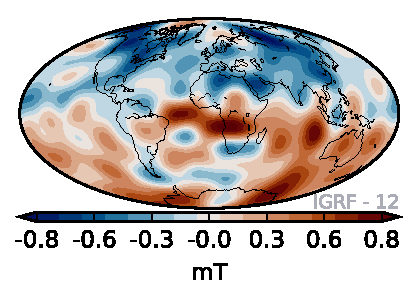
\includegraphics[width=0.4\linewidth]{Terre_B_surf}
		\caption{Composante radiale du champ géomagnétique à la frontière
		noyau-manteau d'après le International Geomagnetic Reference Field
		(IGRF). Les lignes de champ sortent du pôle Sud et rentrent
		dans le pôle Nord.}%
		\label{fig:Terre_surf}
	\end{figure}

	\begin{exemple}
		Le dipôle magnétique est un modèle puissant qui permet de 
		décrire le comportement d'objets micro et macroscopiques. On peut
		donner deux exemples de dipôle magnétique
		\begin{description}
			\item[Le champ magnétique terrestre: ] Le champ magnétique
			 terrestre résulte des déplacements du fluide conducteur
			 qui compose la partie externe du noyau de la Terre.
			 En première approximation, on peut assimiler la Terre 
			 à un dipôle magnétique $m = \unit{8.3 \times 10^{22}}
			 {\ampere \usk \meter \squared}$ placé au centre de cette dernière
			 (voir Fig.~\ref{fig:Terre_surf})
			 et présentant un angle de $\unit{11}{\degree}$
			 avec l'axe de rotation. Il en résulte un champ
			 magnétique dont l'amplitude atteint $\unit{50}{\micro \tesla}$
			 à la surface.
			 Attention, le pôle Nord magnétique
			 correspond en fait au pôle Sud d'un moment magnétique !
			\item[Le magnéton de Bohr: ] Le modèle planétaire de l'atome
			d'hydrogène, vu dans le Chapitre~\ref{chap:electrostatique},
			a été proposé par Bohr et permet d'expliquer en partie le magnétisme
			de la matière. Dans ce modèle, l'électron décrit une trajectoire
			circulaire autour du noyau. Ce système peut elors être considéré
			comme une spire de courant de rayon $r_0 = \unit{52.9}{\pico \meter}$
			et de moment magnétique
						\begin{equation*}
				\mu_B = \dfrac{e \hbar}{2 m_e} \approx 
				\unit{9.27 \times 10^{-24}}{\ampere \usk 
				\meter \squared},
			\end{equation*}
			où $m_e$ est la masse d'un électron, $e$ sa charge en 
			valeur absolue et $\hbar \approx 
			\unit{1.05 \times 10^{-34}}{\joule \usk \second}$ 
			la constante de Planck réduite.
		\end{description}
	\end{exemple}

\subsection{Action d'un champ magnétique extérieur}
Il s'avère qu'un dipôle magnétique $\vecm$ plongé dans un champ magnétique extérieur 
$\vecb$ subit de la part de ce champ une action mécanique sous la forme d'un couple
$\mitbf{\Gamma}$
\begin{defn}[Action d'un champ magnétique sur un dipôle magnétique]
	Soit un dipôle magnétique $\vecm$ plongé dans un champ magnétique $\vecb$.
	Le champ magnétique va exercer un couple $\Gamma$ sur le dipôle tel que
\begin{equation}
	\mitbf{\Gamma} = \vecm \wedge \vecb,
\end{equation}
dont nous admettrons l'expression. 

L'énergie d'interaction $E$ entre un moment dipolaire $\vecm$ et un champ magnétique
$\vecb$ s'écrit
\begin{equation*}
	E = - \vecm \cdot \vecb.
\end{equation*}
\end{defn}

Pour illustrer cette interaction, nous allons 
considérer le cas d'une boussole placée dans le champ magnétique terrestre orienté
selon $\ey$ (voir Fig.~\ref{fig:gamma}). 
\begin{figure}[htpb]
	\centering
	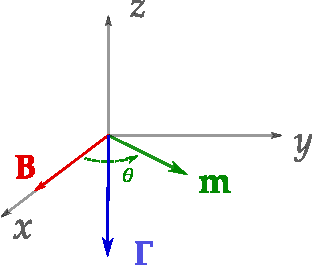
\includegraphics[scale=1]{gamma}
	\caption{Action d'un champ magnétique $\vecb$ sur un dipôle magnétique
	$\vecm$.}
	\label{fig:gamma}
\end{figure}
Initialement,
l'axe de cette boussole présente un axe $\theta$ avec le champ magnétique. Ce dernier
va alors exercer un couple $\mitbf{\Gamma}$ sur l'aiguille de la boussole tel
\begin{equation}
	\mitbf{\Gamma} = -mB\sin\theta \ez.
\end{equation}
Ce couple va alors avoir pour action d'aligner $\vecm$ avec $\vecb$.

\section{Le vecteur aimantation}
Nous allons maintenant voir comment le modèle du dipôle magnétique va nous permettre
de décrire les propriétés magnétiques d'un milieu via son aimantation. Nous allons 
notamment nous concentrer sur le lien qu'il existe entre l'aimantation et 
le champ magnétique.

\subsection{Approche microscopique}
Certains milieux matériels, tels que les aimants, sont capables de générer
des champ magnétiques importants. Ampère suggèra alors que ces champs magnétiques 
étaient créés par des spires microscopiques liées à la structure du matériau.
En réalité, les propriétés magnétiques d'un matériau découlent 
de l'existence de dipôles magnétiques atomiques qui proviennent
\begin{itemize}
	\item d'une part du moment magnétique orbitale résultant du mouvement des 
	  électrons autour du noyau. Nous avons d'ailleurs calculé la valeur de ce moment
	  pour l'atome d'hydrogène dans son état fondamental.
	\item et d'autre part du spin des électrons et des nucléons, 
	  ce dernier étant un moment magnétique intrinsèque à une particule. 
\end{itemize}
Malheureusement, l'étude de l'aimantation microscopique est complexe 
et nécessite de faire appelle à une théorie quantique de la matière, ce qui sort 
totalement du cadre de ce cours. Nous nous limiterons donc ici à une approche macroscopique
de la matière aimantée.

\subsection{Approche macroscopique}
Pour éviter de devoir nous plonger dans une théorie quantique de la matière, nous
allons donc changer d'échelle, en ne regardant plus la matière à l'échelle atomique
mais à une échelle plus élevée. Imaginons que nous voulions décrire les propriétés magnétiques d'un milieu occupant un volume $\mathcal{V}$ de l'espace (voir Fig.~\ref{fig:aimantation}). 
Pour ce faire, nous allons découper
ce volume en $N$ volumes macroscopiques $\{\dV_i\}_{i \in [\![1,N]\!]}$, centrés 
au point $\{P_i\}_{i \in [\![1,N]\!]}$, 
tels que 

\begin{equation*}
\mathcal{V} = \sum_{i = 1}^N \dV_i. 
\end{equation*}
Ces volumes doivent être assez grands 
pour contenir un grand nombre d'atomes mais pas trop grands pour éviter 
que les propriétés physiques à l'intérieur de ce dernier ne varient trop.
Le moment magnétique $\vecd\vecm_i$ 
de chaque volume $\dV_i$ s'obtient alors en sommant la contribution de chaque atome
\begin{equation*}
	\vecd\vecm_i = \sum_j \mathcal{M}_j,
\end{equation*}
où $\mathcal{M}_j$ est le moment magnétique du $j$-ème atome contenue dans 
le volume $\dV_i$.
Si ce volume est assez grand devant les dimensions atomiques, on peut alors
introduire une densité volumique de moment dipolaire $\vecM$ telle que
\begin{equation*}
	\vecd\vecm_i = \vecM(P_i) \dV_i.
\end{equation*}
$\vecM$ est aussi appelé le vecteur aimantation ou l'aimantation du milieu.

\begin{figure}[]
	\centering
	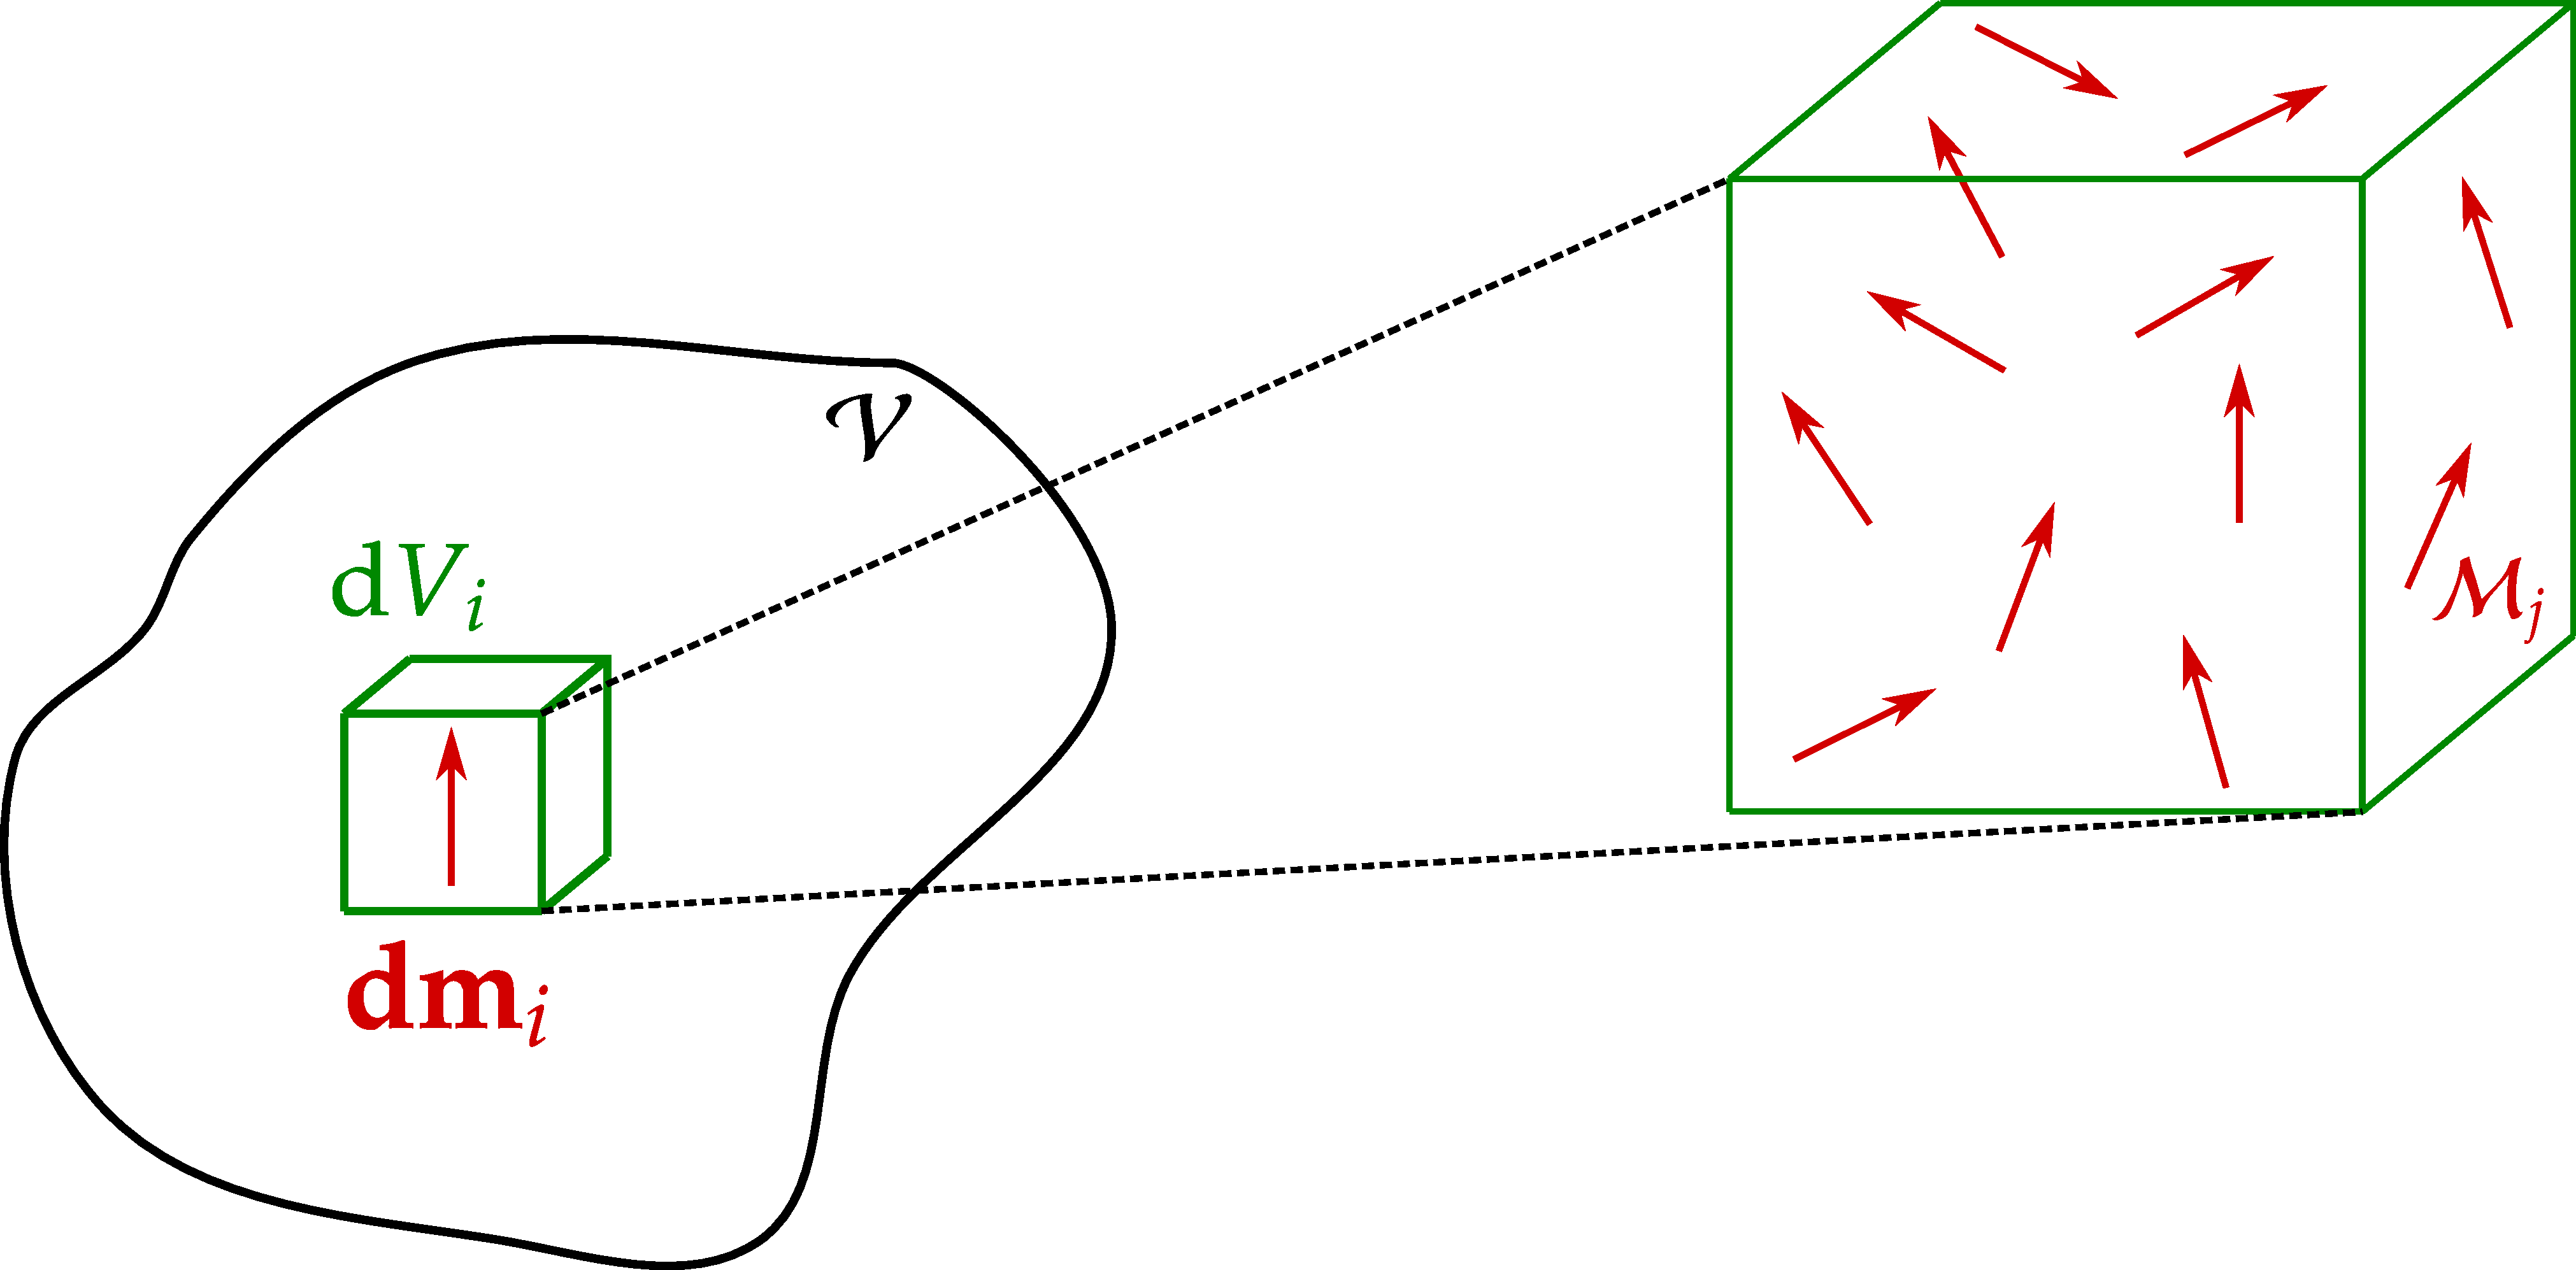
\includegraphics[scale=1]{aimantation}
	\caption{Découpage d'un volume $\mathcal{V}$ en volume macroscopique
	$\dV_i$. Chaque volume $\dV_i$ possède un moment magnétique $\vecd\vecm_i$
	qui résulte de la superposition des moments magnétiques $\mathcal{M}_j$
	des atomes qui le composent.}%
	\label{fig:aimantation}
\end{figure}

\begin{defn}[Vecteur aimantation]
	Soit un petit élément de volume $\dV$ d'un domaine magnétique $\mathcal{V}$.
	Ce volume centré en un point $P$ de l'espace 
	possède un moment dipolaire $\mathrm{\textbf{d}}\vecm$ tel que
	\begin{equation}
		\mathrm{\textbf{d}}\vecm = \vecM(P) \dV,
	\end{equation}
	où $\vecM(P)$ est la densité volumique de moment dipolaire en $P$.
	$\vecM$ est donc un champ vectoriel qu'on appelle aussi vecteur aimantation
	ou aimantation.
	Il s'exprime en $\ampere \usk \reciprocal \meter$.
\end{defn}

La valeur de ce champ vectoriel au point $P_i$ est obtenue en réalisant une
moyenne spatiale des moments dipolaires atomiques inclus dans $\dV_i$
\begin{equation*}
	\vecM(P_i) = \dfrac{\displaystyle{\sum_j \mathcal{M}_j}}{\dV_i}.
\end{equation*}

\subsection{Équivalence entre aimantation et distribution de courant}
À l'échelle macroscopique, il est possible de montrer que rien ne distingue 
un champ magnétique dû à des dipôles magnétiques d'un champ généré par une distribution de
courant. La distribution d'aimantation peut alors être remplacé par une distribution de 
courant équivalente.

Soit un volume $\mathcal{V}$ délimité par une surface $\mathcal{S}$ et
possédant une aimantation $\vecM$. Le champ magnétique généré par ce volume
est équivalent à celui que produirait une distribution de courant caractérisée
par
\begin{itemize}
	\item une densité volumique de courant $\vecj$ à l'intérieur
	  de $\mathcal{V}$ telle que
	  \begin{equation}
		  \vecj = \rot \vecM.
	  \end{equation}
       \item une densité surfacique de courant $\vecj_s$ sur la surface
	 $\mathcal{S}$ telle que
	 \begin{equation}
		 \vecj_s = \vecM \wedge \vecn,
	\end{equation}
	où $\vecn$ est le vecteur unitaire normal à $\mathcal{S}$ et dirigé
	vers l'extérieur de $\mathcal{V}$.
\end{itemize}

En nous appuyant sur cette équivalence, on aboutit alors à une
nouvelle forme de l'équation de Maxwell-Ampère.

\begin{defn}[Champ magnétique et aimantantion]
	Soit un domaine magnétique présentant une aimantation $\vecM$. En l'absence
	de courant électrique, le champ
	$\vecb$ à l'intérieur du domaine vérifie alors la relation
	\begin{equation}
		\rot \vecb = \mu_0 \rot \vecM.
	\end{equation}
\end{defn}

La plupart du temps, à ce champ magnétique créé par l'aimantation $\vecM$ 
vient se superposer
un champ magnétique généré par une densité volumique de courant $\vecj$ . Le champ total
$\vecb$ vérifie alors
\begin{equation}
	\rot \vecb = \mu_0 \vecj + \mu_0 \rot \vecM \iff \rot\left(\dfrac{\vecb}{\mu_0} 
	- \vecM\right) = \vecj.
\end{equation}
Il est alors commode dans ce cas de définir le vecteur excitation magnétique 
$\vecH$.

\begin{defn}[Vecteur excitation magnétique]
	Soit un domaine aimanté $\mathcal{D}$ caractérisé par une aimantation 
	$\vecM$ et
	une densité volumique de courant $\vecj$ qui résulte d'un mouvement 
	de porteurs de charge. Le champ magnétique $\vecb$ 
	à l'intérieur du domaine vérifie alors
	\begin{equation*}
		\rot\left(\dfrac{\vecb}{\mu_0} - \vec{M}\right) = \vecj
		\quad \mathrm{et} \quad \div \vecb = 0.
	\end{equation*}
	On définit alors le vecteur excitation magnétique $\vecH$ tel que
	\begin{equation}
		\vecH = \dfrac{\vecb}{\mu_0} - \vec{M}.
	\end{equation}
	$\vecH$ a la même dimensionnalité que $\vecM$. Il s'exprime donc en 
	$\ampere \usk \reciprocal \meter$. 
\end{defn}	

L'introduction du vecteur d'excitation magnétique $\vecH$ permet d'aboutir
à une nouvelle forme des équations de la magnétostatique.

\begin{defn}[Équation de la magnétostatique et milieux aimantés]
	Soit un domaine aimanté $\mathcal{D}$ caractérisé par une aimantation $\vecM$ et
	une densité volumique de courant $\vecj$ qui résulte du mouvement 
	des porteurs de charge. Le champ magnétique $\vecb$ et 
	l'excitation magnétique $\vecH$ vérifient alors

\begin{equation}
		\div \vecb = 0, \quad \rot \vecH = \vecj \quad \mathrm{avec}
		\quad \vecb = \mu_0 \left(\vecH + \vecM\right).
\end{equation}
Sous forme intégrale, ces égalités deviennent
\begin{equation}
	\oiint_\mathcal{S} \vecb \cdot \ds = 0 \quad \mathrm{et} 
	\quad \oint_\mathcal{C} \vecH \cdot
	\dl = I,
\end{equation}
où $I$ est le courant enlacé par le contour fermé $\mathcal{C}$.
\end{defn}

\section{Aimantation induite}
Contrairement aux aimants, la plupart des 
matériaux ne possèdent pas d'aimantation permanente.
En revanche, sous l'action d'un champ magnétique extérieur, ces derniers vont acquérir 
une aimantation $\vecM$ qui est alors qualifiée \textbf{d'aimantation induite}. 
L'aimantation du matériau en un point est alors une fonction du champ magnétique 
totale $\vecb$ en ce point. La relation qui lie $\vecb$ à $\vecM$ est alors caractéristique du
matériau considéré. Elle décrit la réponse de ce dernier à un champ magnétique externe.
Cette relation constituve découle le plus souvent de résultats expérimentaux.

\subsection{Paramagnétisme, diamagnétisme et ferromagnétisme}
Concernant l'aimantation induite, on distingue alors deux grandes classes de matériaux
\begin{itemize}
	\item Dans la plupart des cas, l'aimantation $\vecM$ découlant du champ 
	  magnétique $\vecb$ est faible. Le champ magnétique induit par cette aimantation
	  est donc négligeable devant le champ magnétique imposé. L'aimantation
	  induite peut être dans le même sens que le champ imposé, on parle
	  alors de \textbf{paramagnétisme}, ou dans le sens opposé, on parle
	  alors de \textbf{diamagnétisme}.
	\item En revanche, pour certains matériaux, l'aimantation induite
	  va profondément modifier la structure du champ dans lequel elle se trouve.
	  La relation liant le champ magnétique totale à l'aimantation devient 
	  alors complexe. On distingue dans cette catégorie les matériaux 
	  \textbf{ferromagnétiques,
	  ferrimagnétiques et antiferromagnétiques.} Nous ne considérerons pas
	  le cas des matériaux antiferromagnétiques dans ce cours. 
	  \end{itemize}

Les ferrimagnétiques différent des ferromagnétiques par la manière 
dont les moments dipolaires atomiques s'alignent avec le champ magnétique
externe. Néanmoins, ils réagissent 
macroscopiquement de la même manière à un champ magnétique externe.
Nous ne ferons donc pas la distinction entre les deux et parlerons
uniquement de ferromagnétisme.

\begin{exemple}
	Le fer à température ambiante est un exemple de matériau ferromagnétique.
	L'hélium à température ambiante est un gaz diamagnétique et le lithium est
	quant à lui un métal paramagnétique.
\end{exemple}

\subsection{Susceptibilité magnétique et perméabilité magnétique}
Expérimentalement, on constate que dans les matériaux para- et diamagnétiques
l'aimantation $\vecM$ évolue linéairement avec le champ magnétique imposé
$\vecb$. On définit alors un coefficient de proportionnalité entre l'aimantation
$\vecM$ et l'excitation magnétique $\vecH$.

\begin{defn}[Susceptibilté et perméabilité magnétique]
	Soit un matériau paramagnétique ou diamagnétique plongé dans un champ magnétique
	$\vecb$. Le champ magnétique induit une aimantation $\vecM$ dans le matériau
	qui vérifie la relation
	\begin{equation}
		\vecM = \chi_m \vecH,
	\end{equation}
	où $\vecH$ est l'excitation magnétique et $\chi_m$ est un nombre sans
	dimension appelée la \textbf{susceptibilité magnétique}. La susceptibilité
	dépend du matériau considéré. Le tableau ci-dessous
	donne la susceptibilité de métaux et minéraux usuels à température ambiante. 
	Elle est positive pour les matériaux paramagnétiques et négative
	pour les matériaux diamagnétiques. Pour ces matériaux, l'aimantation
	redevient nulle lorsque $\vecH$ est nul.

	\begin{center}
	\begin{tabular}{l|c}
		\textbf{Matériau} & \textbf{Susceptibilité magnétique}  \\\hline
		Quartz 	 & $-1.5 \times 10^{-5}$ \\[0.5em]
		Eau 	 & $-1.2 \times 10^{-5}$ \\[0.5em]
		Grès     & $10^{-5} - 10^{-2}$\\[0.5em]
	\end{tabular}
	\end{center}

	On déduit alors l'expression qui lie le champ magnétique $\vecb$ à
	l'excitation magnétique $\vecH$
	\begin{equation}
		\vecb = \mu_0(\vecM + \vecH) \iff \vecb = \mu_0 (1 + \chi_m)
		\vecH \iff \vecb = \mu H,
	\end{equation}
	où $\mu$ est la perméabilité relative du milieu.
\end{defn}

\begin{rema}
	Il arrive que la perméabilité relative $\mu$ d'un milieu de susceptibilité
	$\chi_m$ soit définie par 
	$\mu = 1 + \chi_m$.
\end{rema}

La relation constitutive reliant $\vecM$ à $\vecH$ est plus compliquée pour les
matériaux ferromagnétiques. En effet, on conserve la notion de susceptibilité
magnétique pour relier ces deux grandeurs mais elle devient
une fonction non triviale de $\vecH$ et atteint des valeurs pouvant aller
jusqu'à $10^6$. $\vecM$ est alors liée de manière 
non linéaire à $\vecH$ et dépend même de l'histoire magnétique
du matériau. Nous allons maintenant nous concentrer sur la relation liant 
$\vecM$ à $\vecH$ pour les matériaux ferromagnétiques.

\subsection{Le lien entre $\vecH$ et $\vecM$ pour les matériaux 
ferromagnétiques}
On considère dans cette partie le cas d'un noyau de fer ferromagnétique placé à l'intérieur 
d'une bobine parcourue par un courant $I$ (voir Fig.~\ref{fig:noyau_fer}). 
La bobine génère un champ magnétique
entraînant ainsi l'aimantation du noyau de fer. Le fer étant un matériau ferromagnétique,
cette aimantation perturbe
le champ magnétique initial. Il en résulte un champ magnétique total 
beaucoup plus important.

\begin{figure}[htpb]
	\centering
	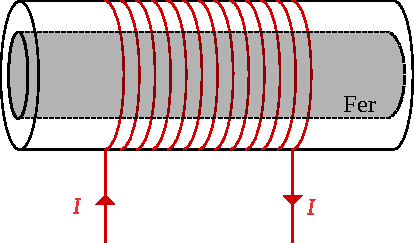
\includegraphics[scale=0.8]{noyau_fer}
	\caption{Bobine parcourue par un courant $I$ et possédant un noyau de
	fer (en gris sur le schéma).}%
	\label{fig:noyau_fer}
\end{figure}

On cherche ici à déterminer le lien entre l'aimantation $\vecM$, l'excitation
magnétique $\vecH$ et le champ magnétique $\vecb$. 
On note ici $M$, $B$ et $H$ les projections de ces vecteurs sur l'axe de la bobine. 
Expérimentalement,
on fait varier $H$ en faisant varier $I$ et on mesure l'aimantation $M$ et 
le champ magnétique $B$ correspondants. On considère ici un matériau vierge de
tout passé magnétique, c'est-à-dire qu'il n'a jamais été aimanté. Initialement,
on a donc $M=0$, $B=0$ et $H=0$. Que se passe-t-il lorsqu'on fait varier l'intensité
du courant ? Pour répondre à cette question on trace l'évolution de $M$ avec
$H$ et de $B$ avec $H$ (voir Fig.~\ref{fig:hysteresis}).

\begin{figure}[htpb]
	\centering
	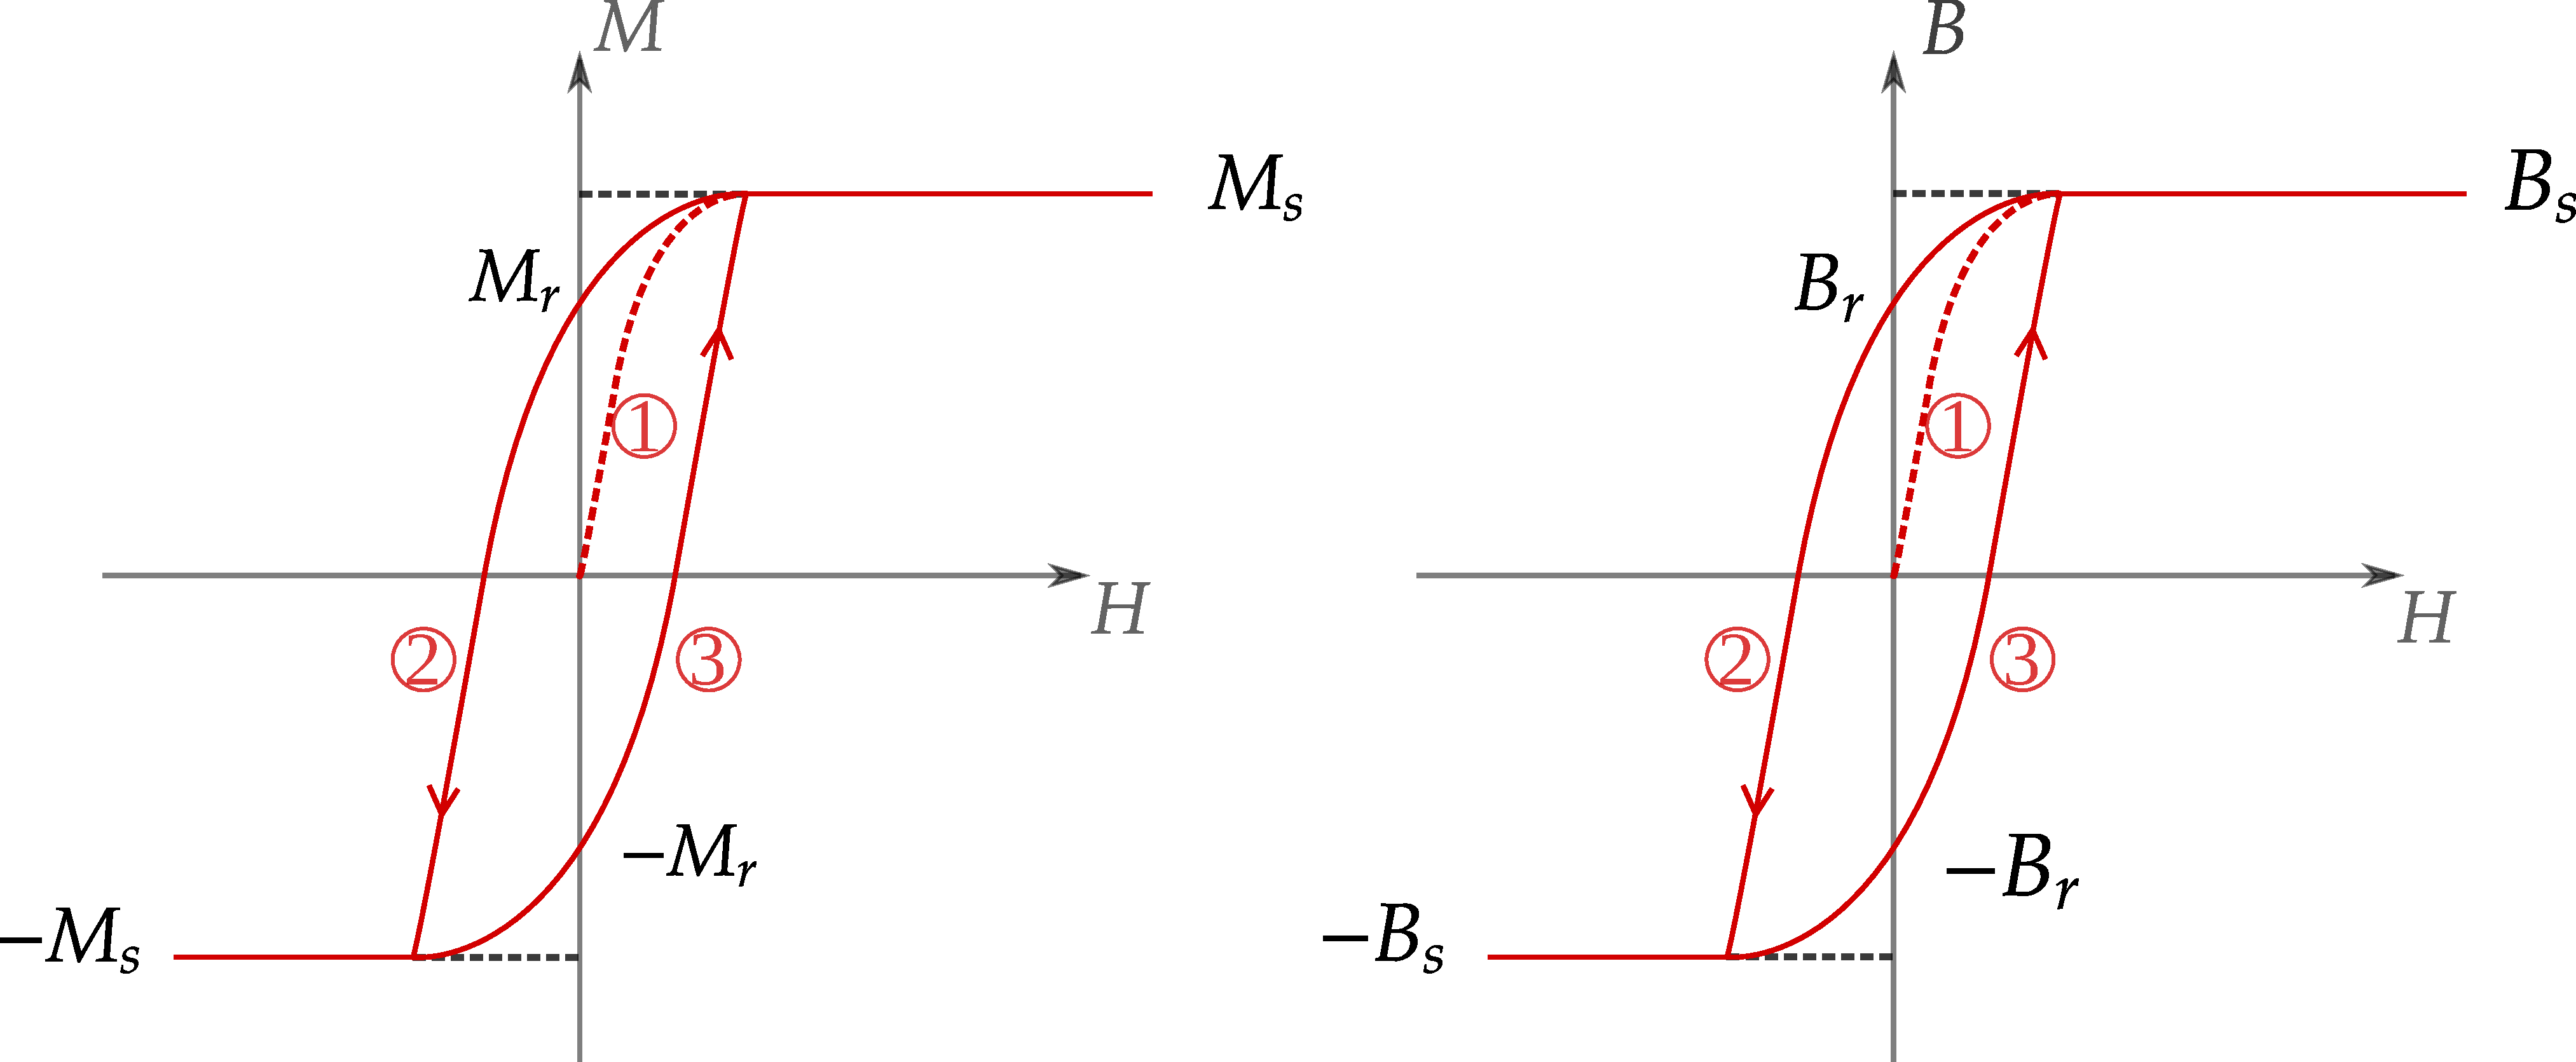
\includegraphics[scale=1]{hysteresis}
	\caption{Évolution de l'amplitude de l'aimantation $M$ (à gauche) et du 
	champ magnétique $B$ (à droite) avec l'amplitude de l'excitation 
	magnétique $H$. Les courbes de première aimantation apparaissent
	en pointillé.}%
	\label{fig:hysteresis}
\end{figure}
\begin{enumerate}
	\item L'augmentation du courant $I$ conduit à un augmentation de $H$.
	  L'amplitude de l'aimantation $M$ et du champ magnétique $B$ croissent
	  de manière non-linéaire avec $H$. Pour des valeurs de $H$ élevées,
	  $M$ et $B$ s'aplatissent et atteignent des valeurs saturées
	  $M_s$ et $B_s$. 
	  La valeur maximale de l'aimantation est appelée \textbf{aimantation 
	  à saturation}. On vient de tracer la courbe de \textbf{première 
  	  aimantation}.
	\item Dans un second temps, on diminue l'intensité du courant et donc
	  la valeur de $H$. Surprise ! Les courbes ne repassent pas par les mêmes 
	  points: l'aimantation du matériau dépend de son passé magnétique !
	  $M$ et $B$ diminuent bien avec $H$ mais il subsiste une 
	  \textbf{aimantation rémanente} $M_r$ et un \textbf{champ magnétique
	  rémanent} $B_r$ lorsque $H = 0$. Le matériau est devenu lui-même
	  un aimant. C'est ce que vous observez après avoir frotté une aiguille
	  contre un aimant. On aboutit finalement à une saturation du matériau
	  qui présente alors une aimantation $-M_s$ et un champ magnétique $-B_s$.
	\item Dans un troisième temps, on augmente de nouveau l'intensité du courant
	  parcourant la bobine. Là encore, les courbes empruntent un chemin 
	  différent, il s'agit du phénomène d'\textbf{hystérésis}.
\end{enumerate}
Le tracé de ce cycle montre à quel point le lien entre aimantation et excitation
magnétique devient complexe pour les matériaux ferromagnétiques. On peut
proposer une explication simplifiée du phénomène pour mieux appréhender ces courbes
d'hystérésis. 

Un matériaux ferromagnétiques est constitués de nombreux domaines, appelés les
domaines de Weiss, dont la taille caractéristique est de l'ordre du $\milli 
\meter$ (voir Fig~\ref{fig:weiss}).
\begin{figure}[htpb]
	\centering
	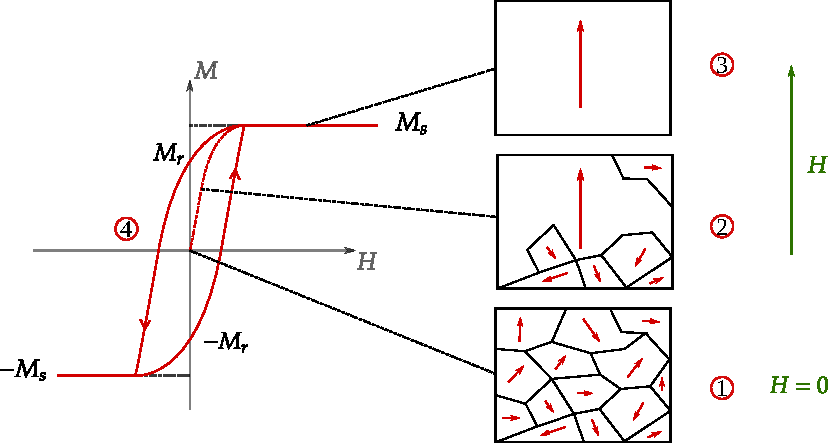
\includegraphics[scale=1]{weiss}
	\caption{Évolution des domaines de Weiss lors du parcours du cycle
	d'hystérésis. Le champ magnétique $\vecb$ appliqué est indiqué par 
	la flèche verte.}%
	\label{fig:weiss}
\end{figure}
Chacun de ses domaines possède un moment magnétique
et génère donc un champ magnétique. 

\begin{enumerate}	
	\item En l'absence de champ magnétique externe,
          les moments dipolaires s'orientent de manière quelconque 
	  sous l'effet de l'agitation thermique. L'ensemble ne présente alors 
	  aucun champ magnétique macroscopique.

  	\item Lorsqu'on applique un champ magnétique externe, 
	  les moments dipolaires vont s'aligner avec ce dernier comme le ferait 
	  une boussole plongée dans le champ magnétique terrestre. 
	  Les domaines étant tous différents, l'alignement des moments
          dipolaires avec le champ extérieur se fait progressivement. Les frontières
	  des domaines se déplacent.
	  
	\item Lorsque tous les domaines pointent dans la même direction, 
	  le matériau est saturé. Son aimantation a atteint la valeur de saturation 
	  $M_s$ (ou $-M_s$). Il est constitué d'un seul domaine de Weiss.

	\item Lorsqu'on diminue l'intensité de $H$, les parois séparant les domaines de 
	Weiss se reconstruisent mais rien ne les oblige à se situer au même endroit que
	précédemment. Cela donne naissance au phénomène d'hystérésis.
\end{enumerate}
Contrairement aux matériaux para- et diamagnétisme, il demeure une aimantation 
rémanente non nulle lorsque $H = 0$ dans les matériaux ferromagnétiques. En effet,
l'interaction entre les moments dipolaires atomiques est plus importante dans ce
type de matériaux et permet ainsi de maintenir une aimantation spontanée.

\section{Étude du champ magnétique terrestre}
\subsection{Transition para-ferromagnétique}
Lorsqu'un matériau para- ou ferromagnétique est soumis à un champ magnétique,
deux phénomènes vont entrer en concurrence. D'un côté, le champ magnétique imposé
tend à aligner les moments dipolaires atomique du matériaux. D'autre part, l'agitation 
thermique entraîne au contraire la fluctuation de l'orientation des moments dipolaires.

Expérimentalement, on constate alors qu'un matériau ferromagnétique
soumis à une température
élevée perd son aimantation spontanée à cause de cette compétition et devient paramagnétique, 
on parle alors d'une \textbf{transition para- ferromagnétique}.
La température à laquelle cette transition survient est appelée la \textbf{température
de Curie}.

\begin{defn}[Transition para-ferromagnétique]
	Un corps ferromagnétique perd son aimantation spontanée et devient 
	paramagnétique lorsqu'il est chauffé à une température supérieure à sa température
	de Curie. Cette température dépend du matériau considéré. Le tableau ci-dessous
	donne sa valeur pour des minéraux et métaux usuels.

	\begin{center}
	\begin{tabular}{l|c}
		\textbf{Matériau} & \textbf{Température de Curie}$\celsius$  \\\hline
		Magnétite 	 & $570$ \\[0.5em]
		Hématite 	 & $650$ \\[0.5em]
		Fer     & $770$\\[0.5em]
		Cobalt     & $1115$\\[0.5em]
	\end{tabular}
	\end{center}
\end{defn}

\begin{rema}
	La température de Curie est spécifique à un matériau. Elle est d'ailleurs parfois
	utilisée pour identifier les minéraux ferromagnétiques qui composent une
	roche.
\end{rema}

\newpage

\subsection{Aimantation thermorémanente}
Une roche est constituée d'un assemblage hétérogène de minéraux. La concentration d'une
roche en minéraux ferrimagnétiques, tel que la magnétite, est souvent faible 
(de l'ordre de $0,01\,\%$ dans le calcaire). Néanmoins, cette faible concentration joue un
rôle primordial dans les propriétés magnétiques de la roche considérée. Notamment
en lui permettant d'acquérir une aimantation rémanente. Lorsque cette dernière
ne résulte pas de l'application d'un champ magnétique externe par un expérimentateur
on parle \textbf{d'aimantation rémanente naturelle}. Cette aimantation est très intéressante
car elle peut donner des informations sur les conditions de formation de la roche
et notamment sur la direction du champ magnétique à cet instant. Elle peut 
résulter de différents phénomènes (sédimentation, éruption, ...). Nous allons
nous concentrer ici sur \textbf{l'aimantation thermorémanente}.

Pour illustrer cela, on considère le cas d'une roche magmatique qui contient une
faible concentration de minéraux ferrimagnétiques, ici de magnétite. 
À la sortie d'un volcan la température de cette roche est supérieure à la température
de Curie de la magnétite qui exhibe alors des propriétés paramagnétiques. 
Bien que cette roche soit soumise au champ magnétique terrestre, l'agitation thermique
rend son aimantation instable en faisant fluctuer la direction des moments magnétiques
atomiques. En revanche, le refroidissement de la roche entraîne une diminution de
l'agitation thermique, les moments dipolaires atomiques tendent alors à s'aligner
avec le champ magnétique externe. Il est alors possible grâce à des procédés 
expérimentaux de retrouver l'orientation du champ magnétique responsable de cette
aimantation rémanente. L'aimantation thermorémanente est particulièrement 
intéressante car elle peut se maintenir sur des temps géologiques et permet
ainsi d'étudier l'évolution du champ magnétique terrestre sur ces mêmes échelles de temps.
Ce type d'étude a notamment permis de montrer que la polarité du champ magnétique 
s'est inversée durant son histoire.

\begin{figure}[h]
	\centering
	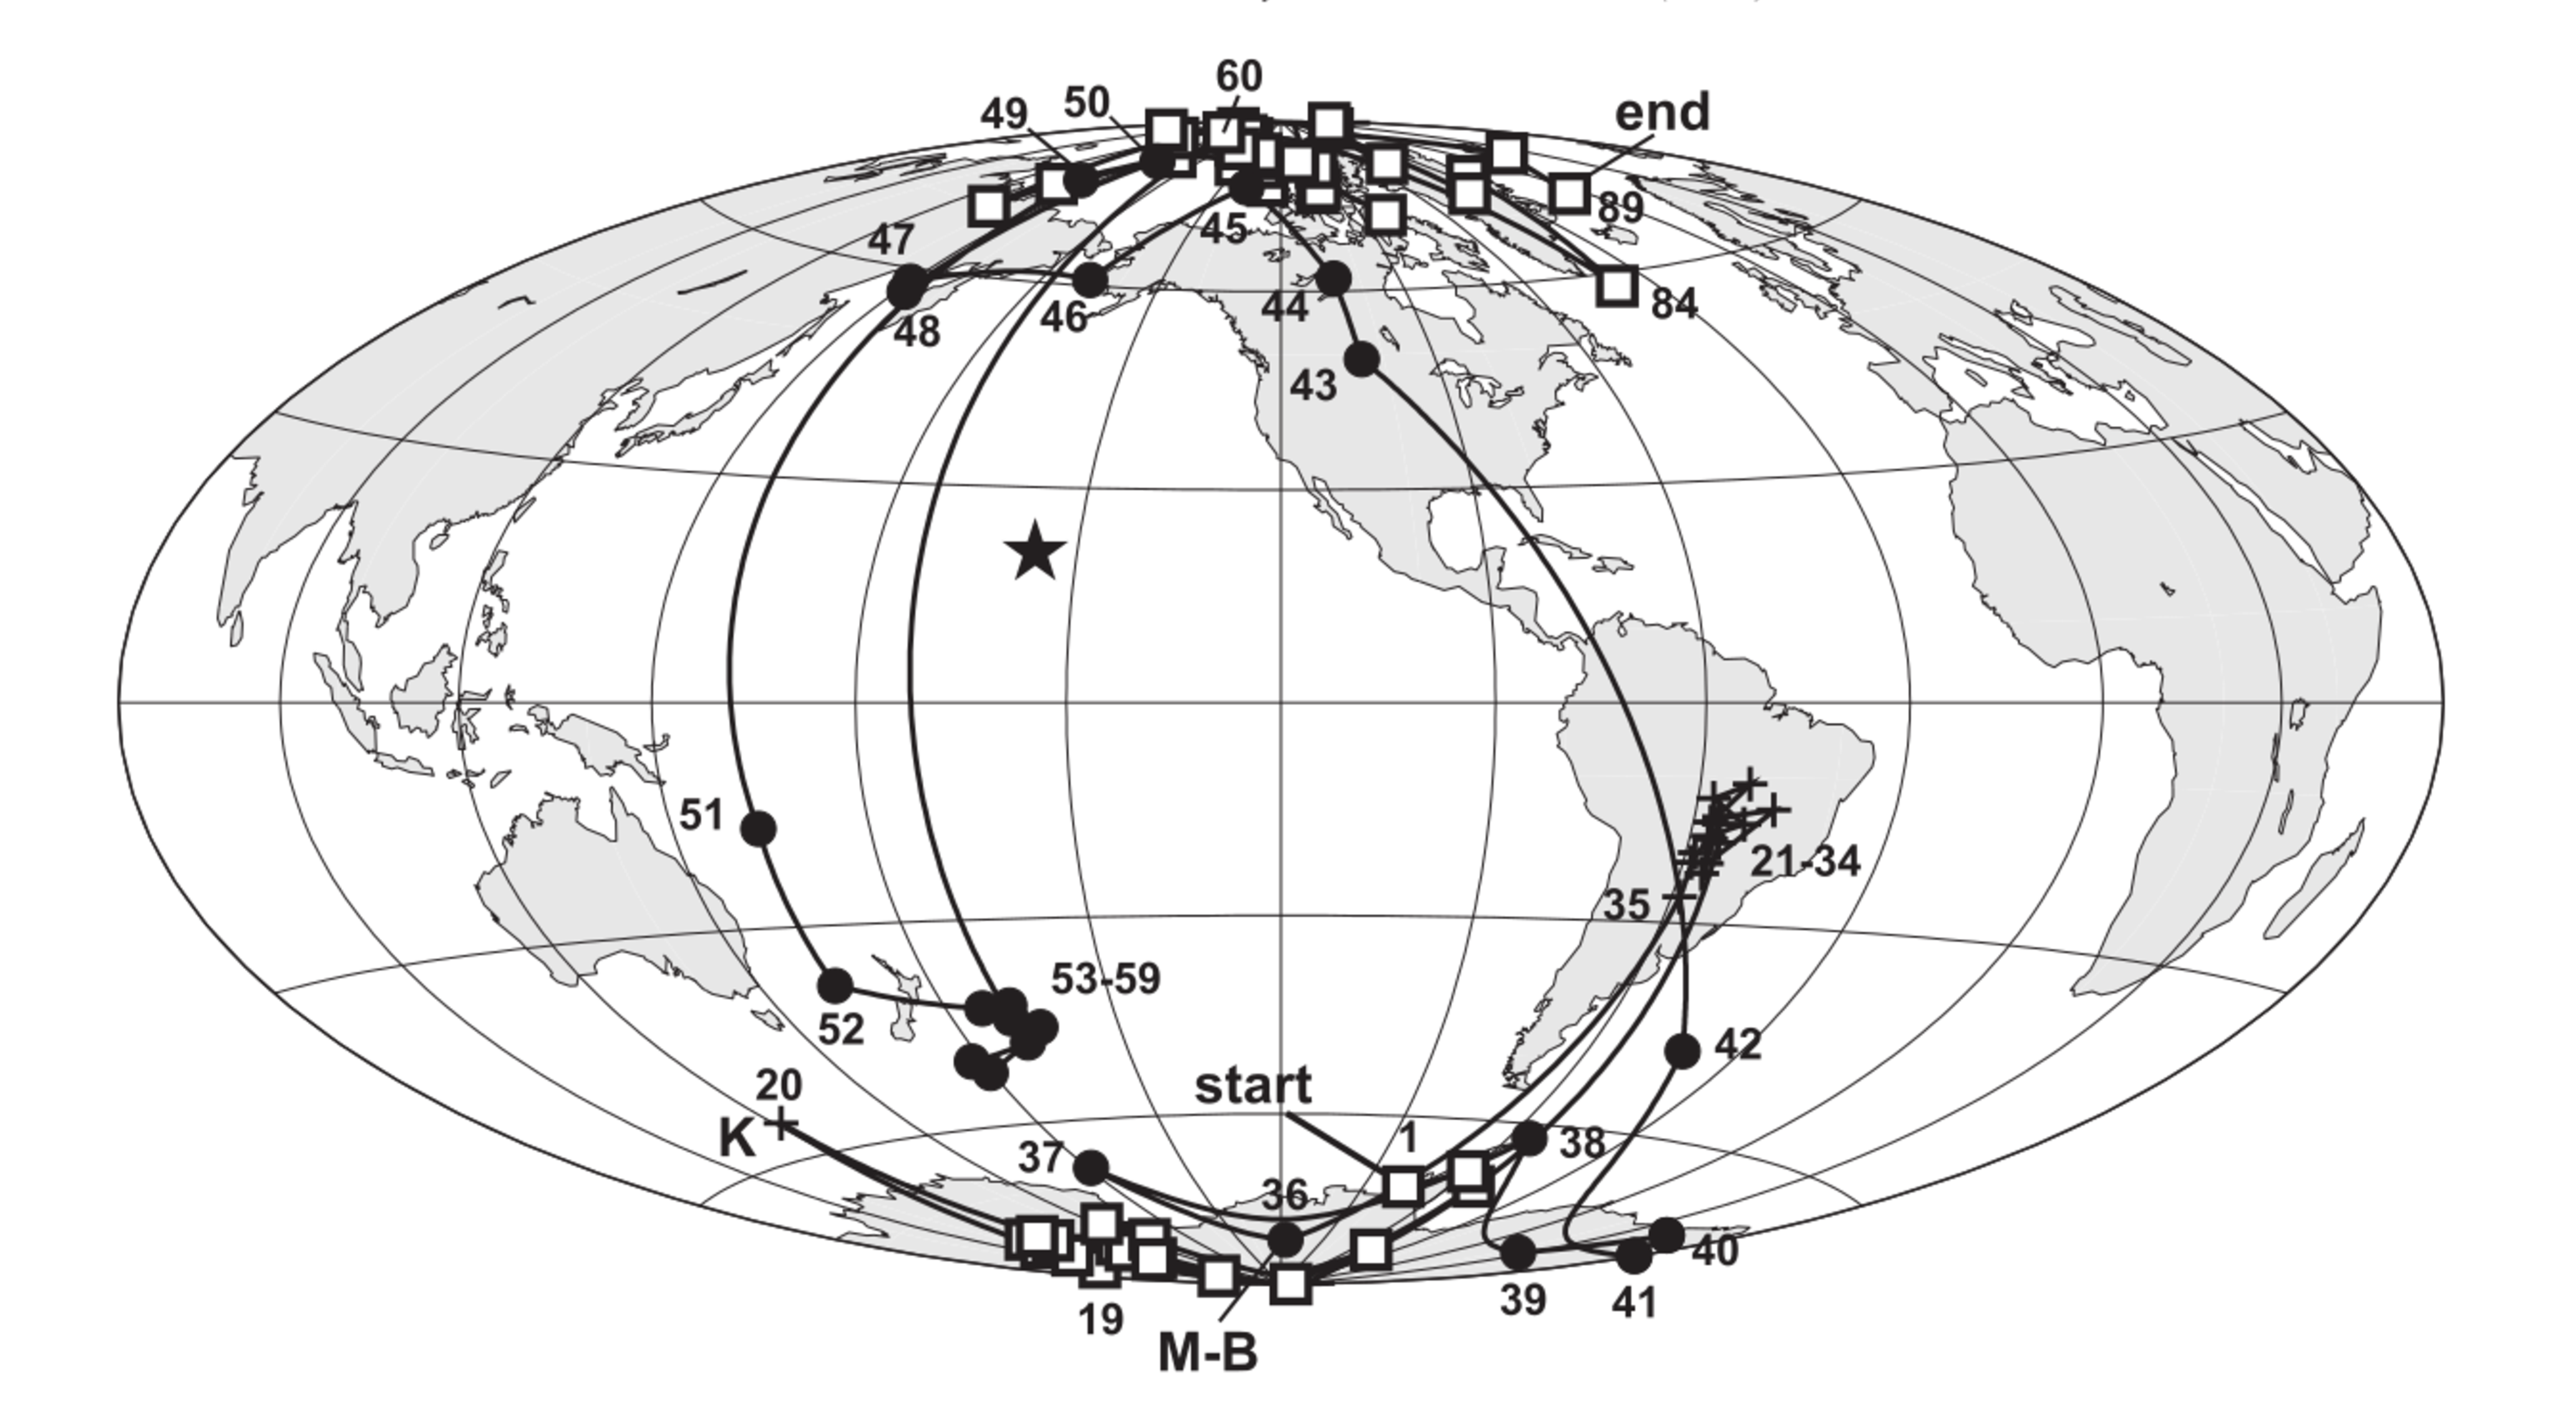
\includegraphics[scale=1]{paleo}
	\caption{Position du pôle Nord magnétique déterminé à partir des
	échantillons de roches magmatiques prélevées sur le volcan Haleakal\=a
	dans l'État d'Hawaï (repéré par une étoile sur la figure). Les carrés
	correspondent aux polarités inverse et normale de Matuyama et de Brunhes. Les
	croix correspondent à un évènement particulier qui a precédé l'inversion, tandis que
	les cercles correspondent à la transition. Cette figure est extraite de 
	\cite{Coe2000}.}%
	\label{fig:paleo}
\end{figure}

\begin{exemple}
	\cite{Coe2000} ont analysé des roches magmatiques provenant de 
	différentes éruptions du volcan Haleakal\=a situé dans l'État d'Hawaï
	(voir étoile sur la figure~\ref{fig:paleo}). Cette étude leur a permis 
	de déterminer
	l'évolution temporelle de la position du pôle Nord magnétique en prélevant des
	roches s'étant formées à différentes époques. Les échantillons utilisés sont
	particulièrement intéressants car ils permettent de visualier une inversion
	de polarité du champ magnétique, appelée l'inversion de Matuyama-Brunhes, 
	qui s'est déroulée il y a $775\ 000$\,ans environ.
\end{exemple}


\begin{rema}
	Nous aurions pu aussi parler d'archéomagnétisme \citep[voir][]{Gallet2009}
	qui s'intéresse au
	champ géomagnétique enregistré par l'aimantation d'artefacts archéologiques
	(briques, four, poterie, ...).
\end{rema}
